% This is samplepaper.tex, a sample chapter demonstrating the
% LLNCS macro package for Springer Computer Science proceedings;
% Version 2.20 of 2017/10/04
%
\documentclass{llncs}
\usepackage{graphicx}
\makeatletter
\@twosidefalse
\@mparswitchfalse
\makeatother
\usepackage{amsmath}
\usepackage{hyperref}
\usepackage{setspace}
\onehalfspacing
\usepackage{float}
\pagestyle{headings}
\setcounter{tocdepth}{8}
\hypersetup{%
    pdfborder = {0 0 0}
}
\renewenvironment{abstract}{%
  \begin{center}%
    {\large\bfseries Abstract}%
  \end{center}%
  \quotation
}{%
  \endquotation
}
\usepackage{appendix}
\usepackage{sectsty}
\sectionfont{\fontsize{15}{14}\selectfont}
\subsectionfont{\fontsize{13}{13}\selectfont}
%
\usepackage{graphicx}
\usepackage[title]{appendix}
% Used for displaying a sample figure. If possible, figure files should
% be included in EPS format.
%
% If you use the hyperref package, please uncomment the following line
% to display URLs in blue roman font according to Springer's eBook style:
% \renewcommand\UrlFont{\color{blue}\rmfamily}


\begin{document}
%

\title{

\begin{figure}[ht]
    \centering
    \includegraphics[width=1\linewidth]{logoENCS.jpeg}
    \label{fig:example}
\end{figure}

Distributed Teams Are Founded on Explicit
Communication Channels\vspace{30pt}}
%
%\titlerunning{Abbreviated paper title}
% If the paper title is too long for the running head, you can set
% an abbreviated paper title here
%

\author{\large \textbf{Het Jatin Dalal - Student ID: 40200513}\vspace{10pt}}
%
%
\institute{\large \textbf{ VCS: Github: \href{https://github.com/Het95/40200513-SOEN6481-TAS}{https://github.com/Het95/40200513-SOEN6481-TAS} \vspace{50pt}\\
\textbf{SOEN 6841- Software Project Management} \\ 
\vspace{15pt} \textbf{Guided by: Prof Pankaj Kamthan \& Iymen Abdella} \\
\vspace{60pt} \textbf{Computer Science and Software Engineering , Concordia University}}}

{\def\addcontentsline#1#2#3{}\maketitle}

\newpage
\begin{abstract}
\large An increase in team size makes it harder to communicate effectively across floors, rooms, cities, or even separate geographical areas. The increased usage of explicit communication channels has thereby improved productivity as well as a number of other aspects of working in a distributed team environment. A team can manage and develop more quickly if written communication is taken into consideration. It also explains how several forms of communication—synchronous, asynchronous, or a mix of the two—are needed to share resources, fill in knowledge gaps, and handle urgent matters. 

\keywords{Explicit communication \and information gaps \and Synchronous \and Ashyncronous \and Distributed team}
\end{abstract}
%
%
%
\tableofcontents
\newpage


%\tableofcontents
%\newpage

\section{ Introduction}
\subsection{ Motivation}

\begin{figure}   
    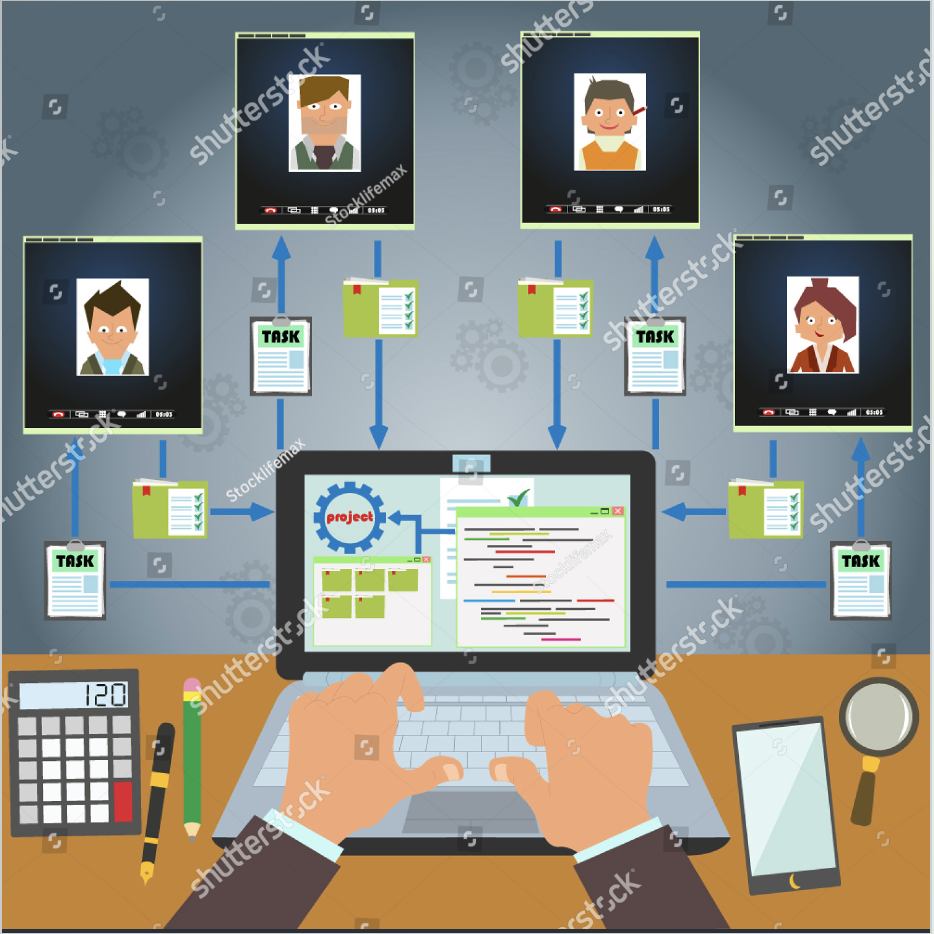
\includegraphics[width=0.2\linewidth]{DTlogo.png}
\end{figure}

The motivation for researching "Distributed Teams Established on Explicit Defined Communication Channels" stems from a number of key considerations and the difficulties of modern work contexts. \\

\begin{enumerate}
    \item \textbf{Surge in popularity of Distributed Team}: The majority of businesses with growing workforces are shifting to distributed team structure, particularly in light of recent pandemics like COVID-19. This makes it much more important in such an environment to collaborate and communicate effectively.~\cite{refbook1}
    \item \textbf{Accountability}: Having clear channels of communication within the team facilitates awareness of individual roles and responsibilities.~\cite{refbook1}
    \item \textbf{Collaboration}: Distributed teams can share project-related materials and do various other project management tasks with each other when they have clear communication channels.~\cite{refbook1}
    \item \textbf{Embrace, Evolve, Adjust}: One must adjust to the changing environment due to changes in new technology, team and company sizes, and the organization can concentrate more on this by employing clear communication channels.~\cite{refbook1}
\end{enumerate}

\subsection{Problem Statement} In distributed team environment, the challenge of effective communication has emerged due to its larger size. Interruptions for resource retrieval is causing productivity loss, especially when team members are intently focused. The necessity for well-defined communication channels has evolved, accompanied by disputes over the advantages of synchronous versus asynchronous systems. There is a need to build a culture of written communication to avoid information gaps and to decisively identify and implement clear and effective communication channels in distributed team environment in order to unlock quick growth and better productivity.~\cite{refbook1}

\subsection{Objectives}
In this investigation, the key objective of the analysis is to describe the significance of using clear and explicit communication channels within distant work environments to boost productivity, efficiency, reducing interruptions, fill information gaps while also allowing them to grow faster. The ultimate objective is to elevate team performance to a new level, promote alignment, preparing teams to work remotely and build resilient teams that can adjust to change.This will help to simplify project management, particularly when adding new team members, and will be advantageous to managers, team leaders, and team members alike. ~\cite{refbook1} 

\section{Background Material}
For the context of the report, it is important to know all the following terms and opinions generated in methodologies section from following case studies in order to gain proper understanding.

\subsection{Terminologies}
 \begin{itemize}
    \item \textbf{Distributed/Remote Teams}: The Distributed Team is spread over the same rooms, city, and possibly even continent. In a nutshell, it consists of two or more people who do not share the same physical workspace or geographical location.~\cite{refbook1}\\
    \item \textbf{Communication Challenges}: Team members' productivity may suffer if they are unclear about where to obtain information or how to communicate well. They could squander time attempting to find information or cause their teammates needless disruptions. causing tap on the shoulder or chat app notifications, when working in deep focus mode ~\cite{refbook1}\\
    \item \textbf{Synchronous \& Asynchronous communication channels}: 
    Synchronous communication channels, which primarily include voice messages, video conferencing apps, instant messaging apps, and in-person meetings if dispersed nearby, can be used to facilitate real-time dialogue between various team members from all walks of life, from information technology to hospitals~\cite{refbook1}~\cite{refpaper1}.
    Asynchronous communication channels , which primarily include collaborative documents like Google Docs, forums, task tracking applications like Jira, Trello, and emails~\cite{refpaper2}, can be used to avoid real-time talk and communicate as needed or by deadline.~\cite{refbook1} \\
    \item \textbf{Multichannel chats}: Multicommunication channels are used to connect with two or more people at the same time or as needed i.e synchronously or asynchronously~\cite{refpaper3}, and include group chats such as Slack. They can be more effective if these communication channels are integrated with project management software or document sharing platforms, ensuring that information is immediately accessible to the team.~\cite{refpaper4}\\
    \item \textbf{Computer Mediated Communication}:  Computer Mediated Communication (CMC) refers to "any human interaction, which are symbolic text-based, directed or facilitated over digitally-based technologies" as well as "the method of creating, exchanging and perceiving the information, which aids encode, decode and transmit the messages by means of telecommunication network. It includes the Internet, text messaging on mobile phones, email, instant messaging.~\cite{refpaper5}
\end{itemize}

\subsection{Related Work}
\begin{itemize}
    \item In ~\cite{refpaper8}, it is mentioned that a startup called Snowpatrol used Skype to conduct synchronous communication in order to minimize the time to market for the product introduction. They used Skype for meetings and used its chat feature extensively in their daily activities. They employed chat channels for various themes, resulting in an efficient communication system. Ad hoc chats addressed unique work difficulties, promoting speedy and concentrated talks among distant team members depicting how SkypeTM is integrated into people's work practices and how it has an immediate impact on managerial practices.\\
    \item In ~\cite{refpaper8}, it is discussed how telecommuting and project-related travel could foster a distributed work environment even when the team is based in one location. Manager Martin has established communication guidelines for updating activities and their locations as a result. Because of this non-traditional usage of SkypeTM, there was more transparency, which made it easier for everyone to comprehend each other's responsibilities and allowed for the application of standard managerial procedures for control and coordination. \\ 
    \item In ~\cite{refpaper8}, when Founder Declan sought to relocate to Barcelona for a more favorable climate, the team employed Skype not only for accomplishing specific agendas but also opted to keep communication channels open throughout the day. This unique approach aimed to cultivate a virtual open office environment, fostering a sense of continuous social presence among team members.\\
    \item In ~\cite{refpaper9}, Geosoft, a multinational software development company, operated in multiple locations, resulting in a remote work environment that presented collaboration challenges. They started using Slack as a multicommunication channel to enhance communication. Using qualitative tools like Nvivo and automatic coding, the research environment was chosen to uncover communication patterns and team dynamics during the transition from Yammer and Skype to Slack.
\end{itemize}


\section{Methods \& Methodology}
\subsection{Computer Mediated Asynchronous Communication: "Boosting Workpace Efficiency"}

\begin{itemize}
    \item In distributed environment, the primary cause of lowering productivity or more shoulder tapping during deep attention hours was delays in resource retrieval that resulted in time waste.~\cite{refbook1}. To address this, Computer Mediated Asychronous Communication(CMAC) proves to be effective. CMAC aids in dealing with communication and productivity obstacles along with providing flexibility.~\cite{refpaper6}\\
    \item CMAC facilitates efficient communication, enabling team members to work together without difficulty across various settings and borders. Over the past few decades, the broad adoption of CMAC technologies has increased communication speed, enabling geographically distributed teams and promoting diversity.~\cite{refpaper6}\\
    \item CMAC guarantees that team members can engage from any location by supporting a variety of communication interactions, such as one-to-one, one-to-many, many-to-one, and many-to-many. This improves teamwork and has a good effect on decision-making, communication, and involvement within the team.CMAC acts as a productive memory aid by producing a precise and permanent archived record that promotes individual and group accountability and makes it possible to look back on previous talks and decisions. Overall, it acts a catalyst for positive shifts in team behaviour and decision making.~\cite{refpaper6}
\end{itemize}

\subsection{Empowering Collaboration through Synchronous Communication Channels}

\begin{figure}
    \centering
    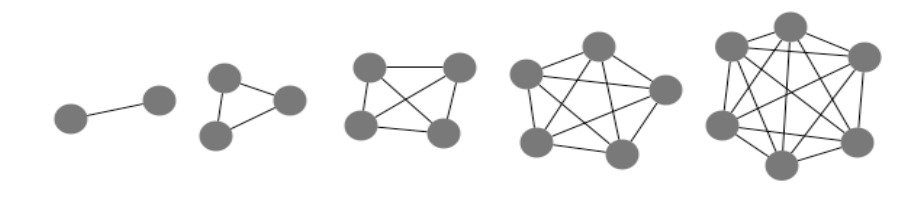
\includegraphics[width=0.9\linewidth]{CommunicationComplexity.png}
    \caption{Overview of communication channel complexity}
    \label{fig:communication-complexity}
\end{figure}

\begin{itemize}
    \item The principal challenge in distributed work environment is  communication complexity especially getting more severe with the increase in team size. As a result, large groups are implicitly conduits for poor communication. The complexity of the channel increases nonlinearly as the number of the team members grows.For instance, A three-person team has three communication channels, while a five-person team has ten, or double the number of people. This is represented in Fig.~\ref{fig:communication-complexity}. ~\cite{refpaper7}. As a result, appropriate synchronous communication channels are needed to carry out communication in efficient manner.~\cite{refpaper7} \\ 
    \item Synchronous communication methods, such as Skype, can facilitate daily meetings and discussions, which can speed up work processes and increase overall productivity. The channels for communication can be arranged according to various subjects, allowing team members to use these impromptu conversations to quickly and easily solve problems that might arise at work. This demonstrates how Skype may improve communication by enabling quicker problem-solving. Furthermore, Skype offers a versatile platform that fosters collaboration and enables independent work, effectively overcoming geographical constraints.~\cite{refpaper8}. \\
    \item The potential of telecommuting and project-related travel could foster a distributed work environment even when the team is based in one location. Implementing clear communication guidelines, such as specifying one's location (e.g., at home or at work) and detailing ongoing activities (e.g., working on a bug), serves as an effective strategy to enhance transparency within the team. This helps in increasing overall efficiency of team.~\cite{refpaper8} \\
\end{itemize}

\subsection{Enhancing Team Dynamics through Multi-Communication Channels}

\begin{itemize}
    \item Multichannel chats have become a important stepping stone for modern communication and distributive environment offering synchronous such as instant messaging or virtual meetings and aynchronous communication such as sharing information.~\cite{refbook1}  \\
    \item The team should establish explicit guidelines or norms for group communication, as everyone's interpretation of norms may differ due to cultural differences. The team should have several types of communication channels dedicated to each perspective, such as frontend, backend, and UX. This helps to avoid unnecessary posting on the general channel, which helps to avoid distraction.~\cite{refpaper9} \\
    \item In conjunction with prioritizing on the main agendas, we can maintain open channels of communication throughout the day to foster a sense of a virtual open office where team members can gather during breaks and engage in small talk to feel socially present. ~\cite{refpaper8}\\
    \item Slack can be used to gather feedback on activities, bridge information gaps, and develop relationships among team members by creating "out of office" communication 
    channels.~\cite{refpaper9}
\end{itemize}


\section{Findings \& Conclusions}

\begin{itemize}
    \item Computer Mediated Asynchronous Communicaiton has helped us how we pursue teamwork, communicaiton and decision making. CMAC teams can communicate, share information, and make decisions in the context of distributed work environment.CMAC teams are easily scalable, allowing for the inclusion of more professionals or the creation of subteams as needed. This flexibility makes it possible for team members to easily share conversations and information electronically, do research, and consult other experts. ~\cite{refpaper6}\\
    \item Skype offered numerous people a way to communicate with CMC. It is an easy and dependable method of conducting synchronous communication. The impact and significance of a technology are not determined by the range of functions it offers. Instead, its usage and influence are shaped by how people choose to use and adopt the technology. Highly innovative approaches have developed around SkypeTM  helping in overcoming  temporal and spatial limitations and providing more detail on the concepts of awareness, availability, and presence.~\cite{refpaper9}\\
    \item It is imperative to establish communication norms and introduce various channels to facilitate teamwork. Using multichannel communication chats, such as Slack, can help to improve teamwork, close information gaps, provide feedback, and improve overall efficiency. ~\cite{refpaper9}

\end{itemize}

\section{Future Work \& Limitations}

\begin{itemize}

\item Even though a sense of social presence was cultivated through open channels, it cannot replace physical touch, and the absence of face-to-face contact makes it challenging to establish personal relationships for effective communication. Additionally, the limitations imposed by internet data caps can further impede seamless communication, affecting response time and task prioritization.~\cite{refpaper8} ~\cite{refpaper9}\\

\item The problem of second language was never considered in distributed environment which could be big factor in creating effective communication among all the team members. ~\cite{refpaper9}\\

\item Most people believed time zones to be the most difficult obstacle because of the enormous time difference. Furthermore, today's economic rivalry necessitates organizations becoming more 'agile' and dynamic in responding to client expectations.~\cite{refpaper10}. \\

\item One difficulty is that text-based communication makes it more difficult to comprehend and control emotions. This is significant because emotional intelligence of team members affects collaboration, and employing chatbots is thought to enhance this.~\cite{refpaper11} \\

\item Conducting comparative studies to evaluate the effectiveness of various communication channels, taking into account factors like team size, industry, and cultural context. This could provide more nuanced recommendations.

\end{itemize}

\bibliographystyle{splncs04}
\begin{thebibliography}{8}
\bibitem{refbook1}
97 Things Every Engineering Manager Should Know [Book],” www.oreilly.com.
\url{https://www.oreilly.com/library/view/97-things-every/9781492050896/}
‌\bibitem{refpaper1}
Coiera, Enrico. "Communication systems in healthcare." Clinical Biochemist Reviews 27.2 (2006): 89.
\bibitem{refpaper2}
Rosen, Benson, Stacie Furst, and Richard Blackburn. "Overcoming barriers to knowledge sharing in virtual teams." Organizational dynamics 36.3 (2007): 259-273
\bibitem{refpaper3}
Mair, Shannon Elizabeth. Two Conversations for One: Synchronous Multimodal Communication. Diss. Georgetown University, 2020.
\bibitem{refpaper4}
Bertram, Dane, et al. "Communication, collaboration, and bugs: the social nature of issue tracking in small, collocated teams." Proceedings of the 2010 ACM conference on Computer supported cooperative work.2010. \url{https://dl.acm.org/doi/10.1145/1718918.1718972}
\bibitem{refpaper5}
Kumar, K. Anil, Subhashree Natarajan, and Biswajit Acharaya. "Computer mediated communication: A pathway to analyze social media communication trajectories." Man in India 97.4 (2017): 195-205.
\bibitem{refpaper6}
Berry, Gregory R. "Can computer-mediated asynchronous communication improve team processes and decision making? Learning from the management literature." The Journal of Business Communication (1973) 43.4 (2006): 344-366. \url{https://doi.org/10.1177/0021943606292352}
\bibitem{refpaper7}
Lalsing, Vikash, Somveer Kishnah, and Sameerchand Pudaruth. "People factors in agile software development and project management." International Journal of Software Engineering \& Applications 3.1 (2012): 117.
\bibitem{refpaper8}
Riemer, Kai, Frank Frößler, and Stefan Klein. "Real time communication-modes of use in distributed teams." (2007)
\bibitem{refpaper9}
Stray, Viktoria, Nils Brede Moe, and Mehdi Noroozi. "Slack me if you can! using enterprise social networking tools in virtual agile teams." 2019 ACM/IEEE 14th International Conference on Global Software Engineering (ICGSE). IEEE, 2019
\bibitem{refpaper10}
Bano, Muneera, Didar Zowghi, and Natalie Sarkissian. "Empirical study of communication structures and barriers in geographically distributed teams." IET software 10.5 (2016): 147-153.
\bibitem{refpaper11}
Benke, Ivo, Michael Thomas Knierim, and Alexander Maedche. "Chatbot-based emotion management for distributed teams: A participatory design study." Proceedings of the ACM on Human-Computer Interaction 4.CSCW2 (2020): 1-30.
\bibitem{reficon1}
“Free Icons,” Icons8.com, 2019. \url{https://icons8.com/icons}

\bibitem{GenAi}
Acknowledgments: chatgpt, perplexity
\end{thebibliography}

\begin{subappendices}
\renewcommand{\thesection}{\Alph{section}}
\section{Images used}
\begin{itemize}
    \item This picture is meant to visually aid the reader's comprehension of a distributed work environment. \url{https://icons8.com/icons}
    \item The communication complexity figure was used to show how communication gets complex with increase in  size
\end{itemize}
\section{Use of Tools}
\begin{itemize}
    \item The overleaf, web based latex IDE  was used for developing latex code which was integrated with Vscode desktop version so that the changes done in overleaf gets reflected in vscode and those changes can then be pushed to github for version control. \url{https://www.overleaf.com/} 
    \item Tools like Grammarly were used for grammer checking and making content more refined.\url{https://www.grammarly.com/}
    \item Generative Artificial Intelligence tools like Chatgpt was used to analyse the case study given for Topic analysis and synthesis \textbf{Example of Some Prompts used}: Difference between Distributed work environment and Remote environment, What is meaning of shoulder tapping, Explain me concept of multichannel chats, summarise me the case study, proof reading and for getting help with latex \url{https://chat.openai.com}
\end{itemize}

\end{subappendices}



\end{document}